\documentclass{beamer}
\usepackage[UTF8]{ctex}
\usepackage{graphicx}
\usepackage{booktabs}
\usepackage{tabularx}
\usepackage{xcolor}
\usepackage{tikz}
\usepackage{hyperref}
\usetikzlibrary{positioning}

\hypersetup{
    colorlinks=true,
    linkcolor=blue,
    urlcolor=blue
}

\title{Ztest: A C++ Unit Testing Framework}
\subtitle{High-level Language Programming Project}
\author{郑辰阳 \quad 叶穗华 \quad 吴泓庆 \quad 齐彦松 \quad 王瑞箐}
\institute{未来技术学院 \\ 数据科学与大数据技术}
\date{2025年6月6日}

\usetheme{Madrid}
\usecolortheme{default}

\begin{document}

\frame{\titlepage}

\section{项目概述}
\begin{frame}{系统背景与动机}
    \begin{itemize}
        \item 面向对象设计与工程实践是软件工程教育的核心
        \item 现有C++测试框架存在不足:
              \begin{itemize}
                  \item 上手难度高
                  \item 缺少原生并发测试运行
                  \item 报告系统简单
                  \item 缺少数据驱动测试
                  \item 与AI技术发展结合不紧密
              \end{itemize}
        \item 我们需要一个:
              \begin{itemize}
                  \item 灵活高效的测试工具
                  \item 支持GUI界面和CLI接口
                  \item 原生支持的测试并发运行
                  \item 多种测试类型(面向并发的两类测试,Benchmark测试,参数化测试)
                  \item 详细测试报告
                  \item AI智能诊断
              \end{itemize}
    \end{itemize}
\end{frame}

\begin{frame}{框架对比}
    \begin{table}
        \centering
        \caption{主流测试框架对比}
        \begin{tabularx}{\textwidth}{lXXXXX}
            \toprule
            \textbf{框架}     & \textbf{GUI支持} & \textbf{并发测试} & \textbf{报告系统} & \textbf{扩展性} & \textbf{数据驱动} \\
            \midrule
            Google Test     & 无              & 有限            & 基础            & 中等           & 不支持           \\
            JUnit           & Eclipse插件      & 支持            & HTML/XML      & 高            & 支持            \\
            PyTest          & 第三方工具          & 优秀            & 丰富            & 优秀           & 支持            \\
            Catch2          & 无              & 一般            & 简洁            & 中等           & 不支持           \\
            \textbf{Ztest*} & 精美             & 优秀            & 丰富            & 高            & 支持            \\
            \bottomrule
        \end{tabularx}
    \end{table}
\end{frame}

\section{系统设计}
\begin{frame}{系统功能}
    \begin{figure}
        \centering
        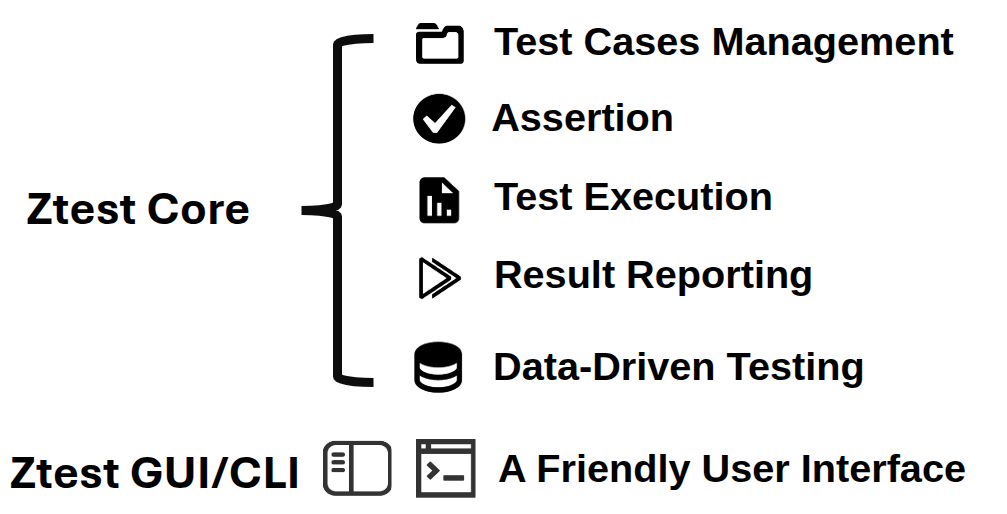
\includegraphics[width=0.8\textwidth]{img/func.png}
        \caption{Ztest功能架构}
    \end{figure}
\end{frame}

\begin{frame}{测试类型}
    \begin{figure}
        \centering
        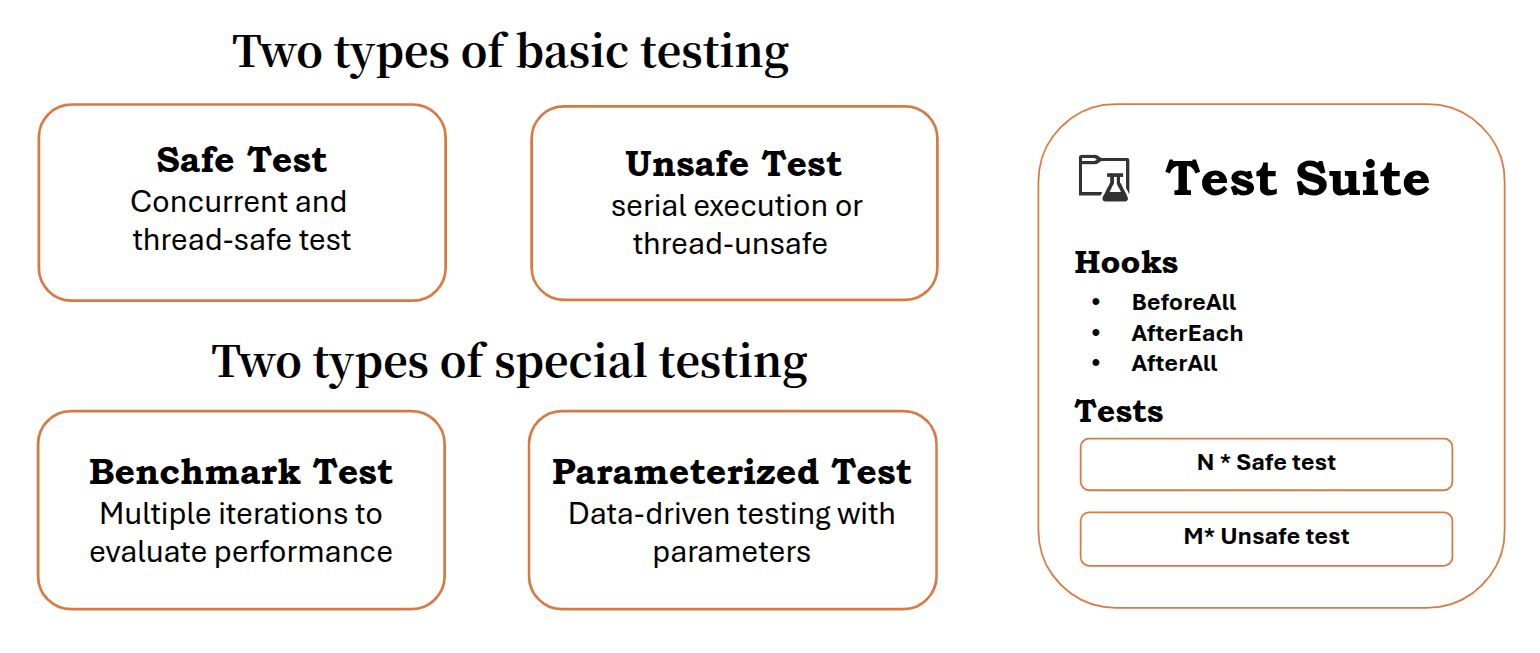
\includegraphics[width=0.8\textwidth]{img/types.png}
        \caption{支持的测试类型}
    \end{figure}
\end{frame}

% \begin{frame}{核心架构}
%     \begin{figure}
%         \centering
%         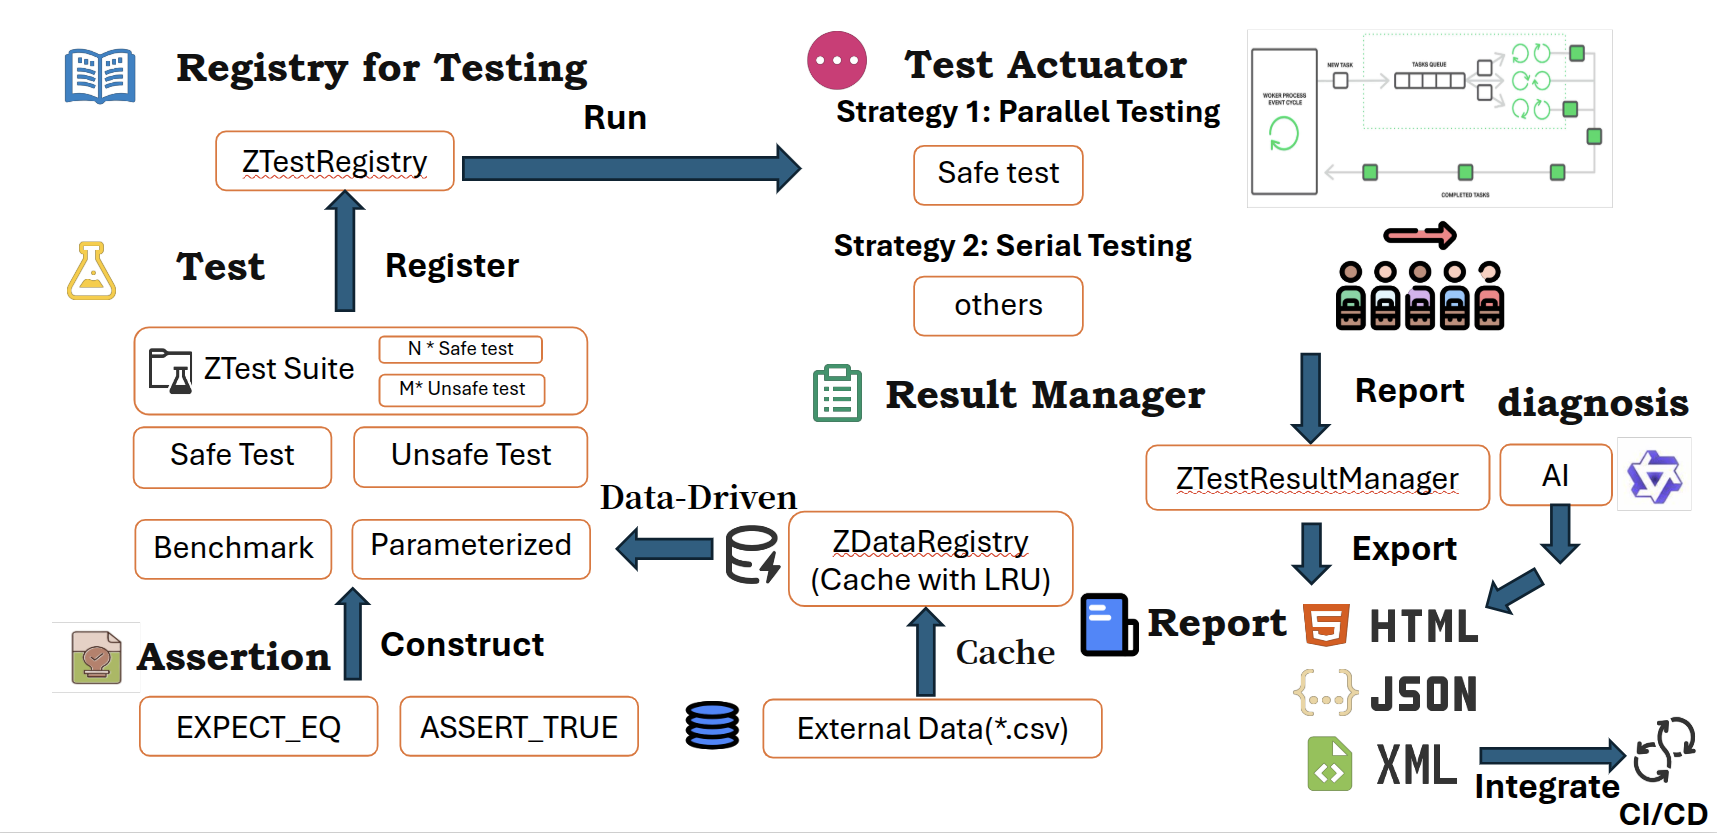
\includegraphics[width=\textwidth]{img/core.png}
%         \caption{Ztest核心架构}
%     \end{figure}
% \end{frame}

% \begin{frame}{GUI架构}
%     \begin{figure}
%         \centering
%         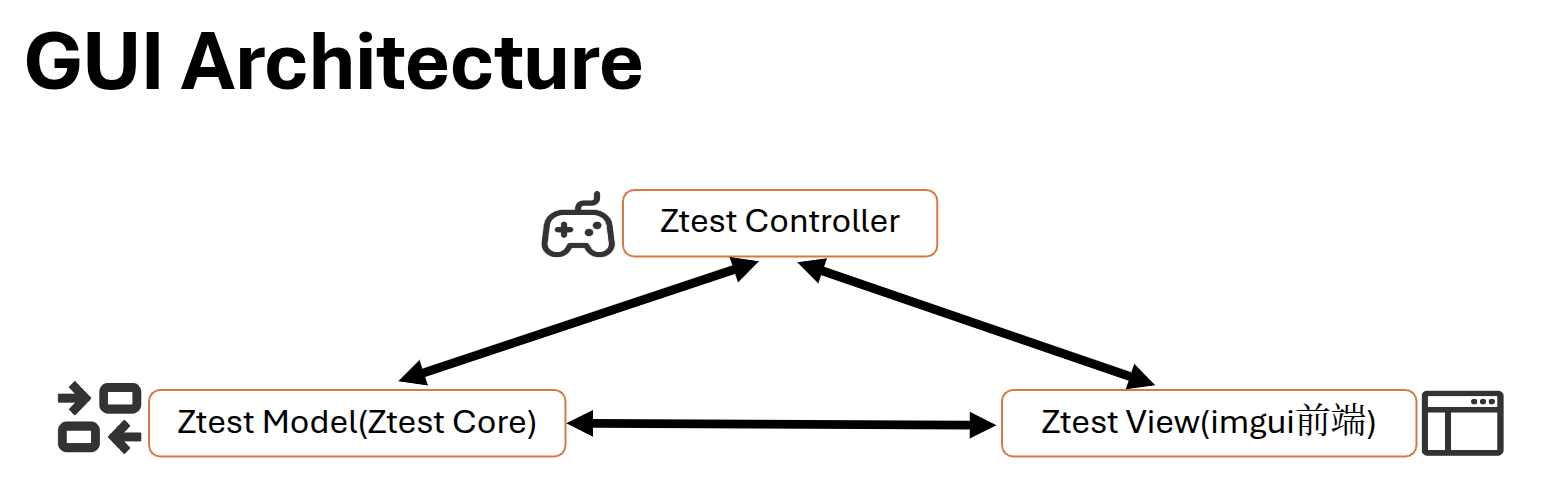
\includegraphics[width=0.8\textwidth]{img/guiarch.png}
%         \caption{GUI架构设计}
%     \end{figure}
% \end{frame}

% \begin{frame}{类图设计}
%     \begin{figure}
%         \centering
%         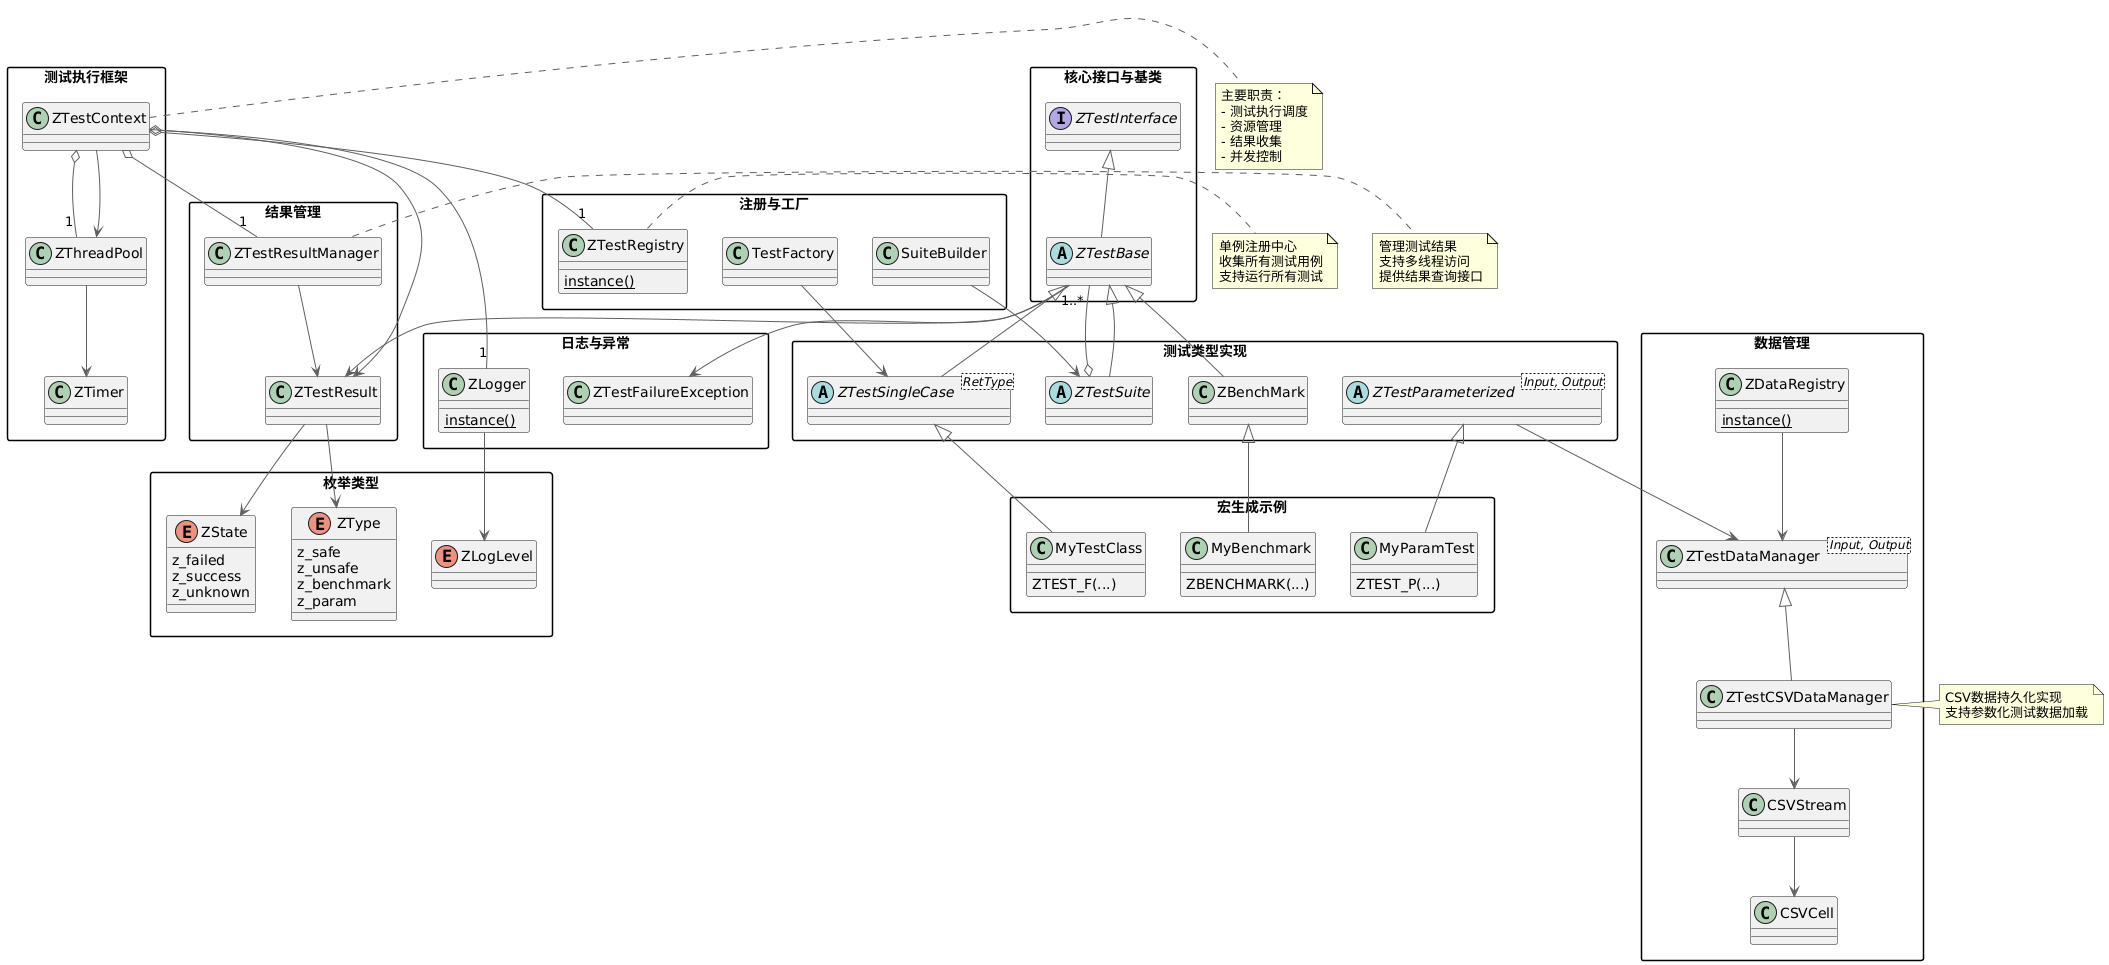
\includegraphics[width=\textwidth]{img/class.png}
%         \caption{系统类图}
%     \end{figure}
% \end{frame}

% \section{关键技术}
% \begin{frame}{测试定义语法}
%     \begin{block}{测试定义宏}
%         \begin{lstlisting}[basicstyle=\ttfamily\small]
% ZTEST_F(SuiteName, TestName, safe/unsafe) { ... }
% ZBENCHMARK(SuiteName, TestName, iterations) { ... }
% ZTEST_P(SuiteName, TestName, data) { ... }
% ZTEST_P_CSV(SuiteName, TestName, "data.csv") { ... }
%         \end{lstlisting}
%     \end{block}

%     \begin{block}{链式定义}
%         \begin{lstlisting}[basicstyle=\ttfamily\small]
% auto test_case = TestFactory::createTest("Add", ZType::Z_SAFE, "", add, 2, 3)
%                  .setExpectedOutput(5)
%                  .beforeAll([]() { logger.info("Init\n"); })          
%                  .afterEach([]() { logger.info("Clean\n"); }).build();
%         \end{lstlisting}
%     \end{block}
% \end{frame}

% \begin{frame}{断言机制}
%     \begin{itemize}
%         \item \textbf{EXPECT\_EQ}: 验证两个值是否相等
%         \item \textbf{ASSERT\_TRUE}: 验证条件是否为真
%     \end{itemize}

%     \begin{exampleblock}{使用示例}
%         \begin{lstlisting}[basicstyle=\ttfamily\small]
% EXPECT_EQ(5, add(2, 3));
% ASSERT_TRUE(6==add(2, 3));
%         \end{lstlisting}
%     \end{exampleblock}

%     \begin{alertblock}{异常处理}
%         断言失败抛出 \textbf{ZTestFailureException},可自定义异常处理
%     \end{alertblock}
% \end{frame}

% \begin{frame}{数据驱动测试}
%     \begin{itemize}
%         \item 参数化测试支持
%         \item CSV数据导入
%         \item 数据缓存优化:
%               \begin{itemize}
%                   \item 懒加载机制
%                   \item LRU缓存淘汰策略
%               \end{itemize}
%     \end{itemize}

%     \begin{exampleblock}{示例代码}
%         \begin{lstlisting}[basicstyle=\ttfamily\small]
% ZTestDataManager<vector<int>, int> sum_test_data = {
%     {{1, 2}, 3}, {{-1, 1}, 0}, {{10, 20}, 30}};
% ZTEST_P(ArithmeticSuite, SumTest, sum_test_data) {
%   auto &&[inputs, expected] = _data.current();
%   int actual = inputs[0] + inputs[1];
%   EXPECT_EQ_FOREACH(expected, actual);
%   return ZState::z_success;
% }
%         \end{lstlisting}
%     \end{exampleblock}
% \end{frame}

% \begin{frame}{测试执行器}
%     \begin{itemize}
%         \item 多线程并行执行
%         \item 线程池管理
%         \item 智能调度策略:
%               \begin{itemize}
%                   \item 并行运行safe测试
%                   \item 串行运行unsafe测试
%                   \item 串行运行Benchmark
%                   \item 串行运行Parameterized测试
%               \end{itemize}
%     \end{itemize}

%     \begin{figure}
%         \centering
%         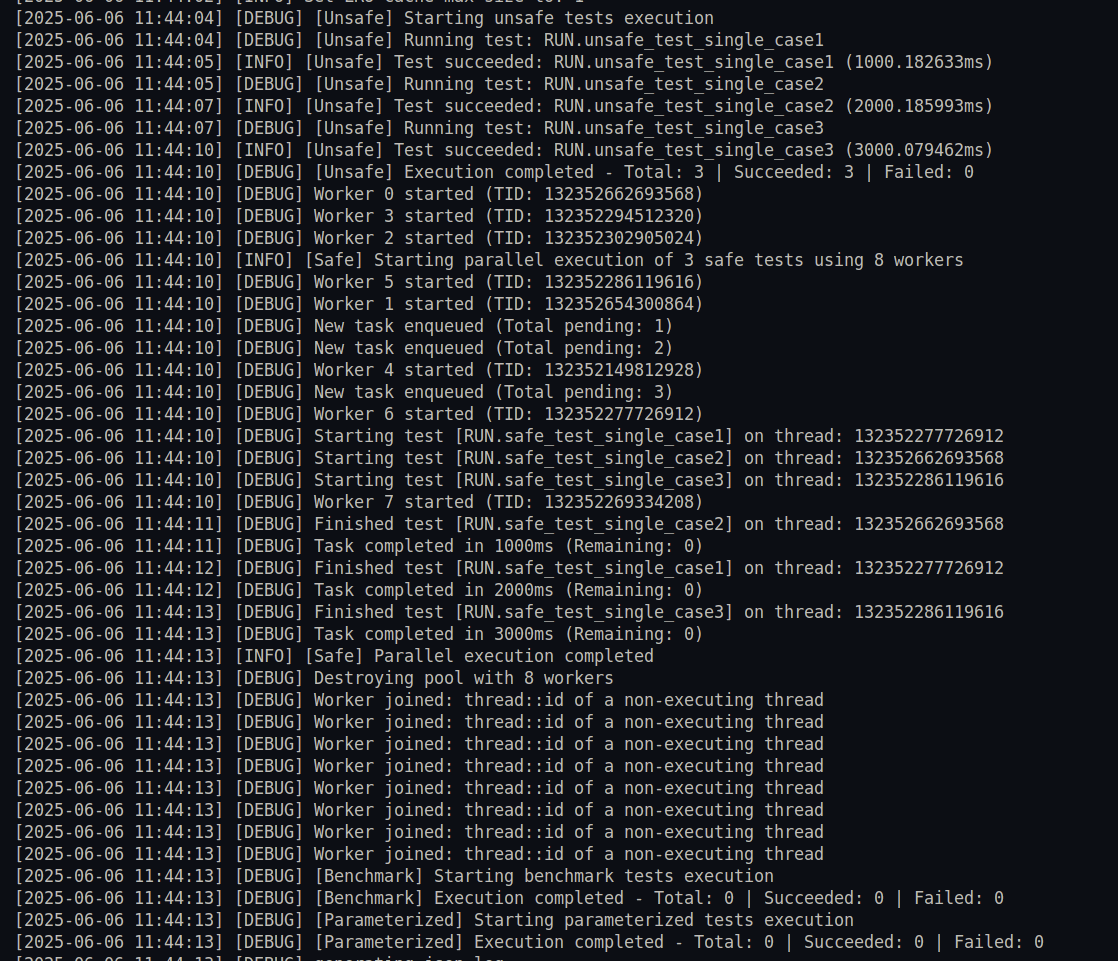
\includegraphics[width=0.8\textwidth]{img/context.png}
%         \caption{测试执行器工作流程}
%     \end{figure}
% \end{frame}

% \begin{frame}{GUI界面}
%     \begin{figure}
%         \centering
%         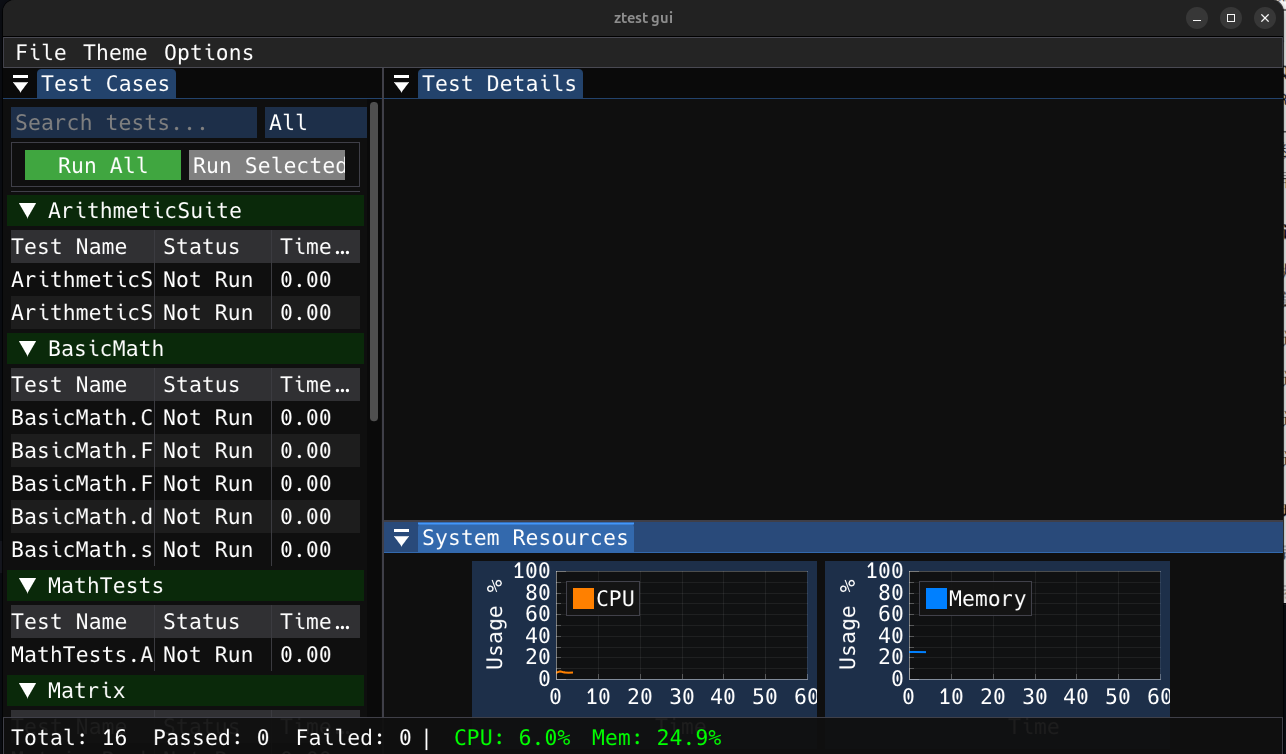
\includegraphics[width=0.8\textwidth]{img/gui.png}
%         \caption{GUI界面设计}
%     \end{figure}
% \end{frame}

% \begin{frame}{AI智能诊断}
%     \begin{columns}
%         \begin{column}{0.5\textwidth}
%             \begin{itemize}
%                 \item 基于qwen3接口
%                 \item 功能:
%                       \begin{itemize}
%                           \item 识别失败原因
%                           \item 提供修复建议
%                           \item 风险评估
%                           \item 覆盖率分析
%                           \item 稳定性建议
%                       \end{itemize}
%             \end{itemize}
%         \end{column}
%         \begin{column}{0.5\textwidth}
%             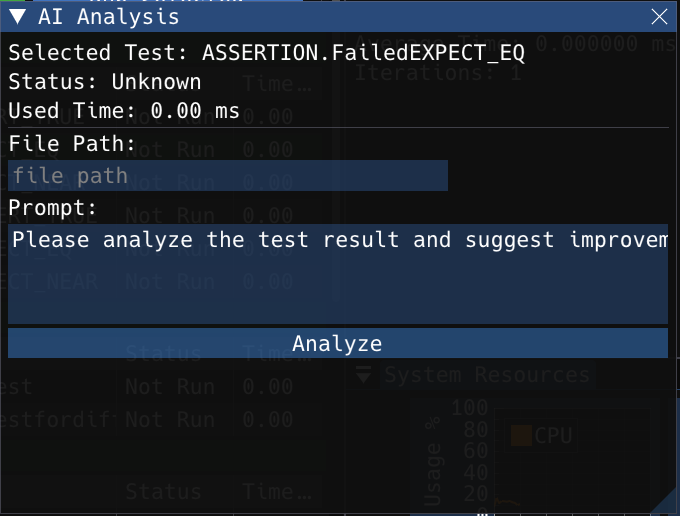
\includegraphics[width=\textwidth]{img/aih.png}
%         \end{column}
%     \end{columns}
% \end{frame}

% \section{测试与成果}
% \begin{frame}{功能测试}
%     \begin{itemize}
%         \item 断言功能测试
%         \item 测试管理测试
%         \item 执行器测试
%         \item 数据驱动测试
%         \item Benchmark测试
%     \end{itemize}

%     \begin{figure}
%         \centering
%         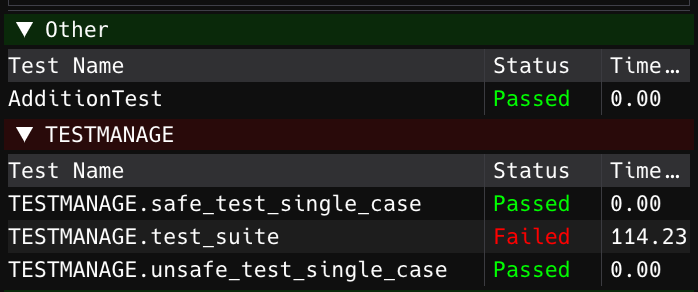
\includegraphics[width=0.6\textwidth]{img/manage.png}
%         \caption{测试管理功能验证}
%     \end{figure}
% \end{frame}

% \begin{frame}{报告生成}
%     \begin{columns}
%         \begin{column}{0.33\textwidth}
%             \centering
%             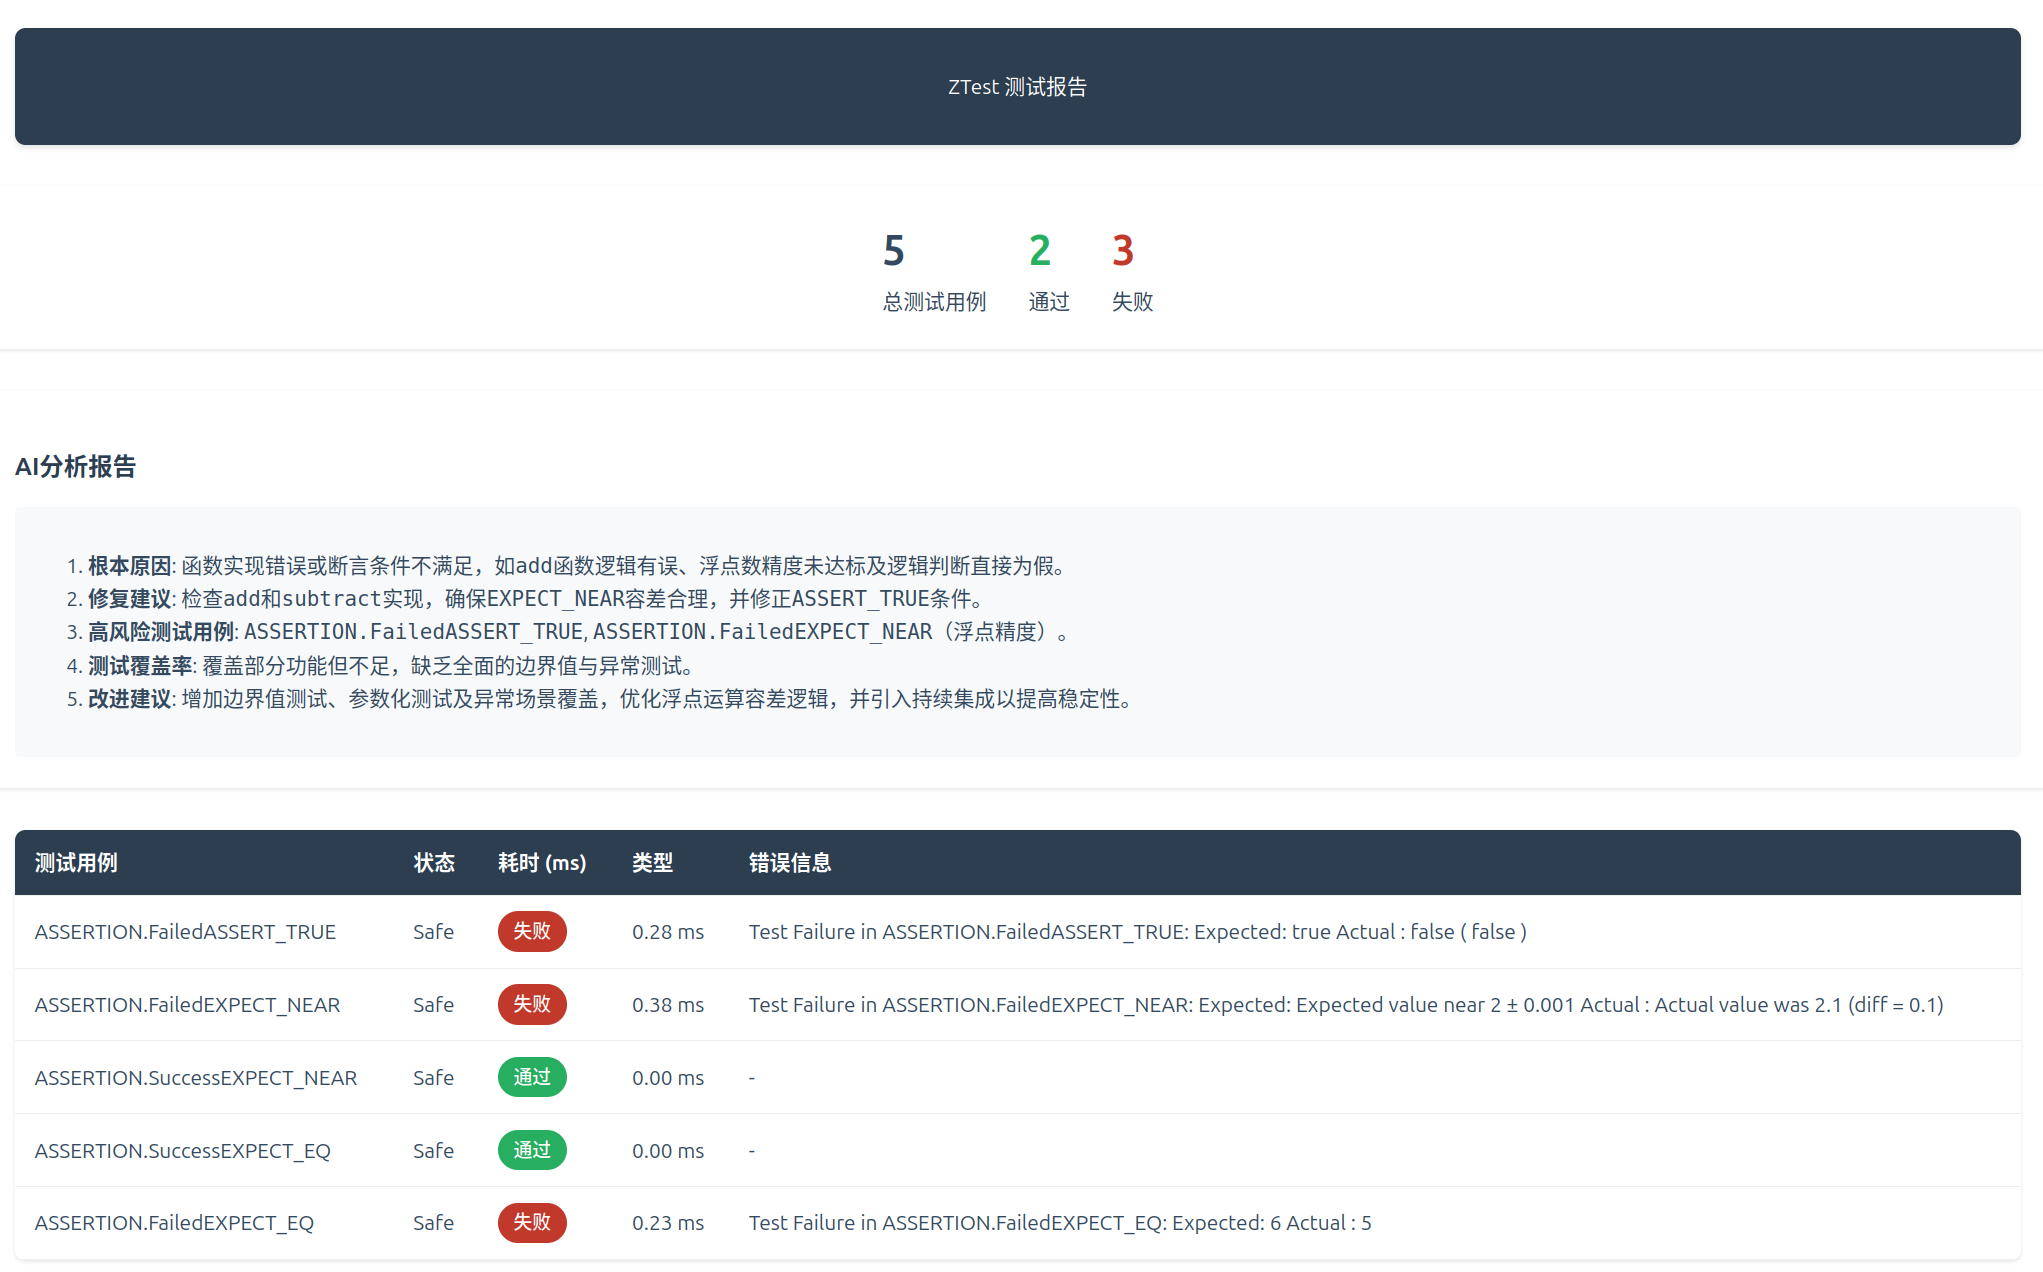
\includegraphics[width=\textwidth]{img/html.png}
%             HTML报告
%         \end{column}
%         \begin{column}{0.33\textwidth}
%             \centering
%             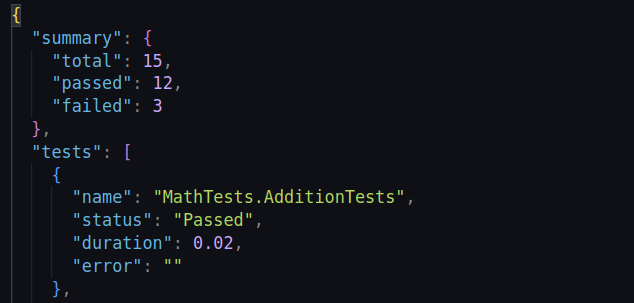
\includegraphics[width=\textwidth]{img/json.png}
%             JSON报告
%         \end{column}
%         \begin{column}{0.33\textwidth}
%             \centering
%             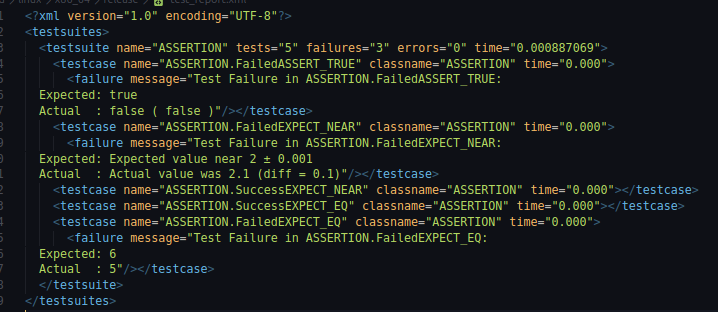
\includegraphics[width=\textwidth]{img/xml.png}
%             XML报告
%         \end{column}
%     \end{columns}
% \end{frame}

% \begin{frame}{开发进度}
%     \begin{table}
%         \centering
%         \begin{tabular}{|l|l|}
%             \hline
%             \textbf{阶段} & \textbf{时间}      \\
%             \hline
%             确定主题        & 2024.04.26-05.03 \\
%             核心代码实现      & 2024.05.03-05.05 \\
%             线程池优化       & 2024.05.05-05.08 \\
%             报告输出实现      & 2024.05.08-05.11 \\
%             GUI改进       & 2024.05.11-05.13 \\
%             CLI接口       & 2024.05.13-05.15 \\
%             Benchmark测试 & 2024.05.15-05.24 \\
%             参数化测试       & 2024.05.25-05.28 \\
%             AI诊断        & 2024.06.02-06.04 \\
%             总结工作        & 2024.06.04-06.05 \\
%             \hline
%         \end{tabular}
%     \end{table}
% \end{frame}

% \section{总结}
% \begin{frame}{团队分工}
%     \begin{table}
%         \centering
%         \begin{tabular}{|l|l|}
%             \hline
%             \textbf{成员} & \textbf{职责}  \\
%             \hline
%             郑辰阳         & 架构设计,核心代码,报告 \\
%             叶穗华         & GUI改进,测试逻辑   \\
%             吴泓庆         & GUI改进        \\
%             齐彦松         & GUI改进        \\
%             王瑞箐         & Windows移植    \\
%             \hline
%         \end{tabular}
%     \end{table}
% \end{frame}

% \begin{frame}{心得体会}
%     \begin{itemize}
%         \item 郑辰阳:深刻体会模块化设计和分层架构重要性
%         \item 叶穗华:前端设计需考虑跨平台、库版本等因素
%         \item 齐彦松:认识到优秀软件需兼顾技术深度和用户体验
%         \item 王瑞箐:实践中学习,收获众多知识
%         \item 吴泓庆:掌握MVC架构实践运用,提高团队合作能力
%     \end{itemize}
% \end{frame}

% \begin{frame}{Q \& A}
%     \centering
%     \Large 谢谢聆听!\\
%     \vspace{1em}
%     欢迎提问!
% \end{frame}

\end{document}